% Source for the figure of the decision tree of the binary search (sec.
% 6.2): the vector of 7 items and the tree whose root is its middle item,
% each node labelled by the place it compares. Build: make figures (in
% ../build).
\documentclass[border=4pt]{standalone}
\usepackage[T1]{fontenc}
\usepackage{lmodern}
\usepackage{amsmath,amssymb}
\usepackage{tikz}
\usepackage{lamalunga}
% tikz-ads.tex: the TikZ styles shared by the figures of the memory of the
% manual, \input by each standalone figure: a cell of a vector (cell), the
% cell that an operation touches (touched), a free cell (free), a node of a
% linked structure (node), the labels of indices (index) and of variables
% (var), a pointer (ptr), and \cells and \indices to draw a row of cells.
\usetikzlibrary{arrows.meta,positioning,calc,fit,shapes.multipart}
\definecolor{adsTouched}{RGB}{214,196,236}
\definecolor{adsFree}{RGB}{236,236,236}
\tikzset{
  ads/.style={>={Stealth[length=2mm]},font=\small,
              every node/.append style={inner sep=0pt}},
  cell/.style={draw,minimum width=7mm,minimum height=7mm,
               font=\small\ttfamily,outer sep=0pt},
  touched/.style={cell,fill=adsTouched},
  free/.style={cell,fill=adsFree,text=black!45},
  node/.style={draw,rounded corners=1pt,minimum width=8mm,
               minimum height=6mm,font=\small\ttfamily},
  index/.style={font=\scriptsize\ttfamily,text=black!60},
  var/.style={font=\small\itshape},
  ptr/.style={->,thick}
}
% \cells{name}{x,y}{list}: a row of cells, the first at (x,y), named
% name-0, name-1, ...; each item is text/style, the style one of cell,
% touched and free (e.g., {a/cell,e/touched,/free})
\newcommand{\cells}[3]{%
  \foreach \v/\s [count=\i from 0] in {#3}
    \node[\s] (#1-\i) at ($(#2)+(\i*7mm,0)$) {\v};}
% \indices{name}{n}: the indices 0 .. n-1 under the cells of name
\newcommand{\indices}[2]{%
  \foreach \i in {0,...,\numexpr#2-1\relax}
    \node[index,below=1.2mm of #1-\i] {\i};}

\tikzset{t/.style={circle,draw,minimum size=7mm,font=\small\ttfamily},
  e/.style={thick}}
\begin{document}
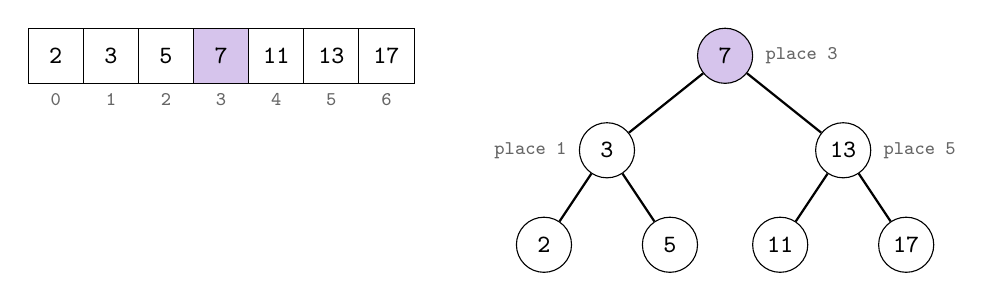
\begin{tikzpicture}[ads]
  \cells{a}{0,0}{2/cell,3/cell,5/cell,7/touched,11/cell,13/cell,17/cell}
  \indices{a}{7}
  \node[t,fill=adsTouched] (r) at (85mm,0) {7};
  \node[t] (l) at (70mm,-12mm) {3}; \node[t] (h) at (100mm,-12mm) {13};
  \node[t] (ll) at (62mm,-24mm) {2}; \node[t] (lh) at (78mm,-24mm) {5};
  \node[t] (hl) at (92mm,-24mm) {11}; \node[t] (hh) at (108mm,-24mm) {17};
  \draw[e] (r) -- (l); \draw[e] (r) -- (h); \draw[e] (l) -- (ll);
  \draw[e] (l) -- (lh); \draw[e] (h) -- (hl); \draw[e] (h) -- (hh);
  \node[index,right=1.5mm of r] {place 3};
  \node[index,left=1.5mm of l] {place 1};
  \node[index,right=1.5mm of h] {place 5};
\end{tikzpicture}
\end{document}
